\documentclass[10pt,landscape,a4paper]{article}

\usepackage[margin=0.225in]{geometry}
\usepackage[utf8]{inputenc}
\usepackage[latin]{babel}
\usepackage[T1]{fontenc}
\usepackage{
  amsmath,
  multicol,
  tabularx,
  listings,
  sectsty,
  lipsum,
  charter,
  dirtytalk,
  graphicx
}

% =============== [ Custom Commands ] ===============
\def\title#1{\hfil{\bf #1}\hfil\par\vskip 2pt\hrule}
\def\cm#1#2{{\tt#1} \dotfill {#2}\\}
% ===================================================

\pdfinfo {
  /Title    (Relational Databases 1)
  /Author   (Rick Daalhuizen)
  /Subject  (KdG TI - Flex 2022-23)
}

\graphicspath{ {images/} }
\pagestyle{empty}
\lstset{language=SQL}
\sectionfont{\fontsize{12}{15}\selectfont}
\setcounter{secnumdepth}{0}
\begin{document}
\begin{multicols*}{3}
  \title{RELATIONAL DATABASES 1}
  \vskip 0.3cm
  
  % ============= [ Content ] =============
  \section{Inleidende Begrippen}
\subsection{Integriteitsregels}
\cm{Key Constraint}{PK moet uniek zijn, en uniek blijven}
\cm{Entity Integrity Constraint}{PK moet geldige waarde hebben}
\cm{Referential Integrity Constraint}{De populatie van FK en PK moet overeenkomen}

\subsection{Bewerkingen met relaties}
\cm{UNION}{RELATIE3 = RELATIE1 $\cup$ RELATIE2}
\cm{INTERSECTION}{RELATIE3 = RELATIE1 $\cap$ RELATIE2}
\cm{VERSCHIL}{RELATIE3 = RELATIE1 $\setminus$ RELATIE2}
\cm{PRODUCT}{RELATIE3 = RELATIE1 $\Pi$ RELATIE2}

\subsection{Eigenschappen van SQL}
\cm{Declaratief}{Instructies wat je wil bereiken}
\cm{Interactief}{Instrcuties en krijg gelijk antwoord}
\cm{Embedded}{Kan het in een programmeertaal gebruiken}

\subsection{Subcategorieën}
\cm{DQL}{$SELECT$}
\cm{DML}{$UPDATE,DELETE,INSERT$}
\cm{DDL}{$CREATE,ALTER,DROP$}
\cm{DCL}{$GRANT, REVOKE$}
\cm{TC}{$COMMIT,ROLLBACK,SAVEPOINT$}

\subsection{Multipliciteiten}
\cm{$0..1$}{Geen of een instantie}
\cm{$1$}{Exact een instantie}
\cm{$*$,$0..*$}{Geen of meerdere instanties}
\cm{$1..*$}{Een of meerdere instanties}
  \section{Select \& Fetch}

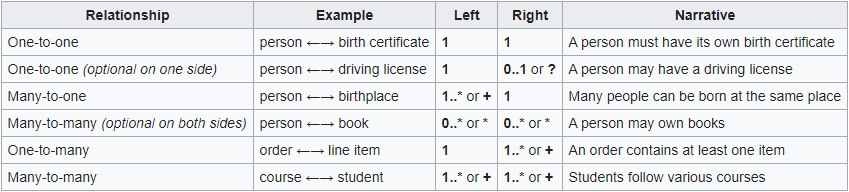
\includegraphics[scale=0.30]{./cardinality.png}

\begin{tiny}
\begin{lstlisting}
SELECT [DISTINCT] select lijst
FROM tabelnaam
[WHERE conditie]
[ORDER BY clausule]
[OFFSET offset ROWS]
[FETCH row limiting clause]
\end{lstlisting}

\begin{lstlisting}
SELECT * FROM employees
WHERE dob
BETWEEN '1-JAN-1980'
AND '31-DEC-1989';
\end{lstlisting}

\begin{lstlisting}
FETCH WITH TIES -- Wanneer je meerdere rijen wilt retourneren die gelijk staan
NULLS FIRST -- Wanneer je NULL waarde als eerst wil tonen
\end{lstlisting}

\begin{lstlisting}
[OFFSET offset ROWS]
FETCH NEXT [row_count]
ROWS [ONLY | WITH TIES]
\end{lstlisting}

\end{tiny}
  \section{Joins}
\say{\(Non\)-Equi-joins, Auto-joins, Date\&Time Functies}

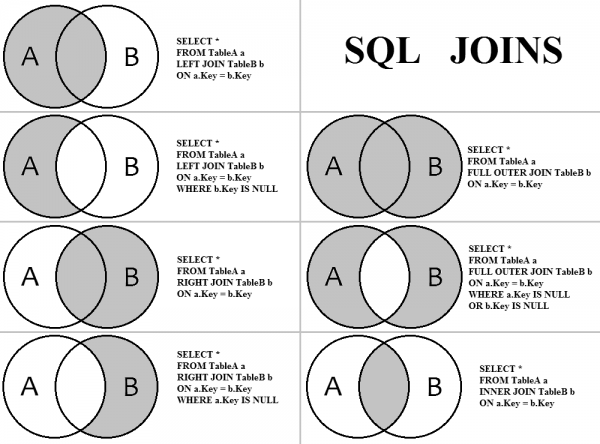
\includegraphics[scale=0.37]{./joins.png}

\subsection{Gewone JOIN}
Resulteert enkel gematchte records.
\begin{tiny}
\begin{lstlisting}
  SELECT * FROM foo f
  [INNER] JOIN bar b -- INNER is default
  ON f.id = b.id
\end{lstlisting}

\begin{lstlisting}
  SELECT * FROM foo
  JOIN bar USING(id) -- kolomnamen hebben dezelfde naam
\end{lstlisting}

\subsection{Non-equi JOIN}
\begin{lstlisting}
  SELECT first_name, last_name, schaalnr
  FROM employees
  JOIN pay_grades ON (salary/12 BETWEEN lower_limit AND upper_limit);

  -- De join is niet gebaseerd op een gelijkheid tussen attribuutwaarden
\end{lstlisting}
\end{tiny}

\subsection{Outer JOIN}
Resulteert in alle gematchte records + null lijnen.

\subsection{Auto JOIN}
Een gewone join, waarbij de tafel met zichzelf samenvoegt.
\say{Oftewel een "recursieve relatie"}

\begin{tiny}
\begin{lstlisting}
  SELECT *
  FROM employees e
  JOIN employees mgr
  ON (e.manager_id=mgr.employee_id);
\end{lstlisting}
\end{tiny}

\subsection{Impliciete conversies}
\cm{cast(foo AS INT)}{Omzetten van tekst naar numeriek}
\cm{to\_char(123, '999')}{Omzetten van numeriek naar tekst}
\cm{to\_char(dob,'TMMonth')}{vertaalde datum naar tekst}

\subsection{Afronden van nummers}
\cm{round(15251.675)}{afgerond op het geheel}
\cm{round(15251.675,1)}{afgerond op 1 decimaal}
\cm{round(15251.675,-1)}{afgerond tot een tiental}

\subsection{Afkappen van nummers}
\cm{trunc(15251.675)}{afgekapt op 1 geheel}
\cm{trunc(15251.675,1)}{afgekapt op 1 decimaal}
\cm{trunc(15251.675,-1)}{afgekapt op 1 tiental}

\subsection{Datum functies}
\cm{current\_date}{huidige datum}
\cm{date\_part}{stuk uit datum halen}
\cm{date\_trunc}{datum afhakken}

\subsection{Leeftijd}
\begin{tiny}
\begin{lstlisting}
  SELECT age(dob) "age" FROM employees;
  SELECT date_part('year',(age(dob))) FROM employees;
\end{lstlisting}

\subsection{Rekenen met datum \& tijd}
\begin{lstlisting}
  SELECT date '2021-09-28' + 7;
  SELECT date '2021-09-28' + interval '10 hour';
  SELECT time '01:00' + interval '3 hours';
  SELECT interval '1 hour' / 1.5;
\end{lstlisting}
\end{tiny}
  \section{Group By \& Outer Join}

\begin{tiny}
\begin{lstlisting}
  -- Geef het hoogste salaris per afdeling:

  SELECT department_id, MAX(salary)
  FROM employees
  GROUP BY department_id
  ORDER BY department_id;
\end{lstlisting}

\begin{lstlisting}
  -- Geef het hoogste salaris per afdeling,
  -- waarvan de waarden kleiner zijn dan 45000:

  SELECT department\_id, MAX(salary)
  FROM employees
  GROUP BY department_id
  HAVING MAX(salary) <45000
\end{lstlisting}
\end{tiny}

\subsection{Analystische functies}
- Geeft 1 RIJ RESULTAAT per groep.\\
- Staan altijd in de $SELECT$ of in de $HAVING$ clausule.\\
- Staan NOOIT in de $WHERE$-clausule!\\
- Houden geen rekening met $NULL$ waarden.\\
\newline
\cm{AVG}{Bereken gemiddelde}
\cm{SUM}{Bereken de som}
\cm{MIN}{Laagste getal}
\cm{MAX}{Hoogste getal}
\cm{COUNT}{Telt attribuutwaarden}

Volgorde van uitvoering:\\
$SELECT -> FROM -> WHERE -> GROUP BY -> HAVING -> ORDER BY$
  \section{Set Operators, Text \& Conditional Functions}

\cm{UNION}{Samenstelling}
\cm{INTERSECT}{Doorsnede}
\cm{EXCEPT}{Verschil}

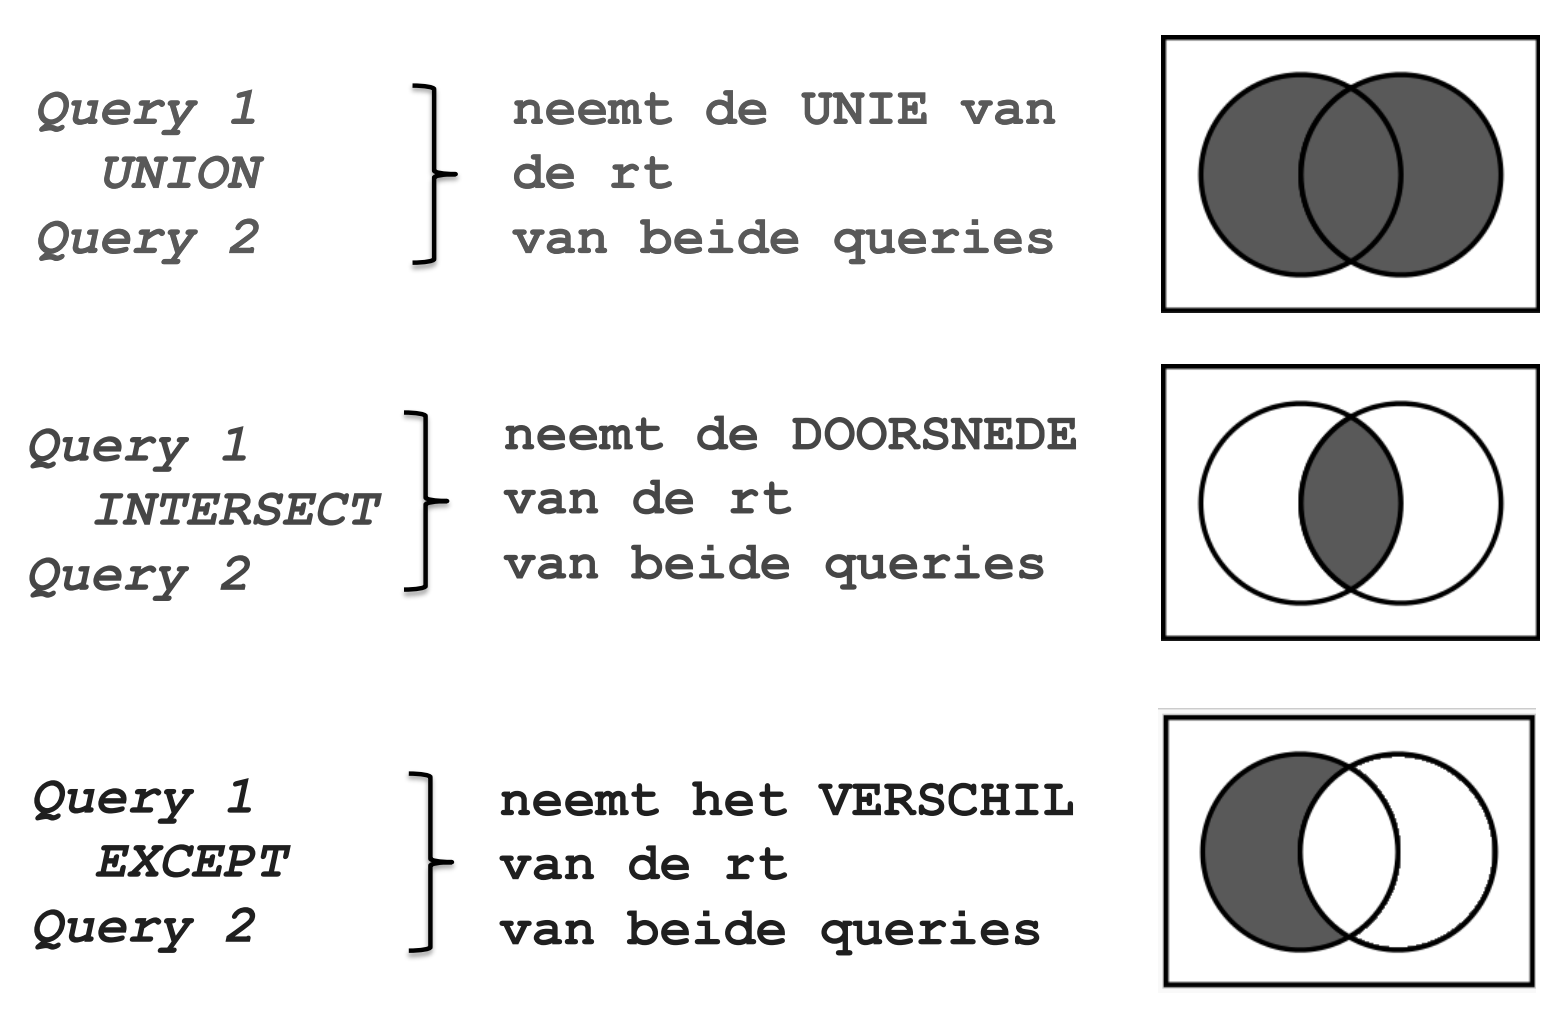
\includegraphics[scale=0.30]{./set-operatoren.png}

\subsection{UNION}
• Plaatst de rijen uit de resultatentabel van de \\
query's samen in één resultatentabel.\\
• Haalt er afhankelijk van het al dan niet aanwezig\\
zijn van de ALL optie, de dubbele rijen tussenuit

\subsection{INTERSECT}
• Plaatst alle rijen van beiden tabellen samen in één\\
resultatentabel.\\
• Haalt er de dubbele rijen tussenuit.\\

\subsection{EXCEPT}
• Plaatst de rijen uit de resultatentabel van de 1e\\
query, die niet voorkomen in de resultatentabel\\
van de 2e query in één resultatentabel.\\
• Haalt er de dubbele rijen tussenuit.\\

\subsection{SET operators combineren}
\begin{lstlisting}
SELECT1 UNION
  (SELECT2 EXCEPT SELECT3)
\end{lstlisting}
  \section{Tekstfuncties}

\cm{UPPER}{Omzetten naar hoofdletters}
\cm{LOWER}{Omzetten naar kleineletters}
\cm{INITCAP}{Beginletter omzetten naar hoofdletter}
\cm{SUBSTR(attr, start, count)}{stuk van tekst}
\cm{POSITION('n' IN attr)}{positie van karakter}
\cm{CONCAT}{tekst aanelkaar plakken}
\cm{LPAD(attr, lenght, fill)}{links aanvullen}
\cm{RPAD(attr, length, fill)}{rechts aanvullen}
\cm{REPLACE(text, from, to)}{karakters vervangen}
\cm{TRIM(TRALING|LEADING|BOTH 'a' FROM attr)}{karakters verwijderen}
  \section{Condtionele functies}

\begin{tiny}
\begin{lstlisting}
  SELECT employee\_id, manager\_id,
  GREATEST(employee\_id, manager\_id),
  LEAST(employee\_id, manager\_id)
  FROM employees;
\end{lstlisting}

\begin{lstlisting}
  SELECT employee_id, province,
    CASE province
      WHEN 'NB' THEN 'Noord Brabant'
      WHEN 'LI' THEN 'Limburg'
      ELSE province
    END "Full name"
  FROM employees;
\end{lstlisting}
\end{tiny}

\subsection{COALSCE}
• De functie geeft de eerste $NOT NULL$ parameter\\
van de parameterlijst terug.\\
• De $COALESCE$ functie heeft minstens 2 parameters\\
• Wanneer alle parameters een $NULL$ waarde bevatten,\\
geeft de functie $NULL$ terug.\\

\begin{tiny}
\begin{lstlisting}
  SELECT COALESCE(hours, 0) FROM tasks;
\end{lstlisting}

\begin{lstlisting}
  SELECT name,
    COALESCE(email, phone, cellphone) contact
  FROM contact_info;
\end{lstlisting}
\end{tiny}

\subsection{NULLIF}
• Geeft NULL terug als beide expressies hetzelfde\\
resultaat geven.\\
• Bij ongelijkheid wordt de eerste parameter teruggegeven.

\begin{tiny}
\begin{lstlisting}
  NULLIF(value1, value2)
\end{lstlisting}
\end{tiny}
  \section{DDL - Create Table}

\begin{tiny}
\begin{lstlisting}
CREATE TABLE tabelnaam(
    attribuutnaam gegevenstype 
		  [default waarde]
		  [column constraint],
    ...,
    [table constraint]
);
\end{lstlisting}
\end{tiny}

\subsection{Constraints}

\cm{PRIMARY KEY}{key constraint + entity integrity constraint}
\cm{NOT NULL}{Mag geen nullwaarde bevatten}
\cm{CHECK}{Moet aan conditie voldoen}
\cm{UNIQUE}{Moet uniek zijn}
\cm{FOREIGN KEY}{referential integrity constraint}
\cm{ON DELETE}{CASCADE / SET NULL}

\subsection{Gegevenstype}
\cm{CHAR|VARCHAR}{Alfanumerieke attributen}
\cm{NUMERIC(n,m)}{Getallen}
\cm{DATE}{Datum zonder tijd}
\cm{TIME}{Tijd zonder datum}
\cm{TIMESTAMP}{Datum en tijd}
\cm{INTERVAL}{Tijd interval}
\newline
\say{Gebruik het datatype CHAR(n) enkel wanneer je zeker weet
dat de attribuutwaarden een vaste lengte hebben}
  \section{DDL - Alter, Drop, Sequence}

\cm{INSERT}{Gegevens invoegen}
\cm{UPDATE}{Gegevens wijzigen}
\cm{DELETE}{Gegevens verwijderen}
\cm{TRUNCATE}{Tabellen leegmaken}
\cm{DROP}{Objecten verwijderen}
\cm{ALTER}{Objecten wijzigen}
\cm{ALTER ADD COLUMN|CONSTRAINT}{aan tabel toevoegen}
\cm{ALTER DROP COLUMN|CONSTRAINT}{van tabel verwijderen}
\cm{ALTER RENAME COLUMN|CONSTRAINT}{van tabel hernoemen}

\begin{tiny}
\begin{lstlisting}
  INSERT INTO foo (foo, bar) VALUES (a, b);
\end{lstlisting}

\begin{lstlisting}
  UPDATE tabelnaam
  SET attribuutnaam=nieuwe waarde
  WHERE conditie;
\end{lstlisting}

\begin{lstlisting}
  DELETE FROM deps USING emp
  WHERE deps.emp_id=emp.id
  AND lower(name)='bob';
\end{lstlisting}
\end{tiny}

\subsection{Sequence}
\say{Wordt gebruikt om automatisch volgnummers te genereren.}

\begin{tiny}
\begin{lstlisting}
  CREATE SEQUENCE [IF NOT EXISTS] sequencenaam
  INCREMENT [BY ] increment
  [MINVALUE minvalue | NO MINVALUE]
  [MAXVALUE maxvalue| NO MAXVALUE]
  [START [WITH] startwaarde
  [CACHE cache]
  [[NO] CYCLE]
\end{lstlisting}

\begin{lstlisting}
  CREATE SEQUENCE seq_project_id
  START WITH 100 INCREMENT BY 5;
  -- 100 105 110 115 120...

  INSERT INTO projects
  VALUES ( nextval('seq_project_id'), 'Foo Bar');
\end{lstlisting}
\end{tiny}
  \section{Subqueries}
Een subquery is een query in een andere query.
\\
• Wordt eerst de subquery uitgevoerd.\\
• Levert waarden aan de hoofdquery.\\

\begin{tiny}
\begin{lstlisting}
  SELECT *
  FROM emplyoees
  WHERE salary = (
    SELECT MIN(salary) FROM employees
  );
\end{lstlisting}
\end{tiny}
\say{Eerst wordt de binnenste $SELECT$ uitgevoerd,\\
daarna de buitenste
}
\\\\
Waar kan je subquery schrijven?\\
$SELECT, FROM, WHERE, HAVING$
\\\\
Subqueries die meer dan 1 rij opleveren\\
\cm{$<ANY$}{Minder dan het hoogste}
\cm{$>ANY$}{Meer dan de laagste}
\cm{$=ANY$}{gelijk aan één van de resultaten}
\cm{$!=ANY$}{verschillend van één van de resultaten}
\cm{$>ALL$}{Meer dan de hoogste}
\cm{$<ALL$}{Minder dan de laagste}
\cm{$<>ALL$}{verschillend van alle resultaten}
\\
Alternatief:
\cm{$<MAX$}{Minder dan het hoogste}
\cm{$>MIN$}{Meer dan de laagste}
\cm{$IN$}{gelijk aan één van de resultaten}
\cm{$>MAX$}{Meer dan de hoogste}
\cm{$<MIN$}{Minder dan de laagste}
\cm{$NOT IN$}{verschillend van alle resultaten}

\subsection{Views}
Via een view kan men gegevens van de\\
onderliggende tabel afschermen.

\begin{tiny}
\begin{lstlisting}
  CREATE OR REPLACE VIEW v_dept_view
    AS SELECT department_id,department_name
      FROM DEPARTMENTS
      ORDER BY department_id;
\end{lstlisting}
\end{tiny}
  \section{Correlated Subqueries}
Er is een ‘correlatie’ (= samenhang) tussen beide queries.
\\
• Daarna levert de subquery informatie aan de hoofdquery.\\
• Levert de hoofdquery eerst informatie aan de subquery.\\

\begin{tiny}
\begin{lstlisting}
  SELECT employee_id, last_name, department_id
  FROM employees e
  WHERE NOT EXISTS (
    SELECT 'x'
    FROM employees
    WHERE manager_id = e.employee_id
  );
\end{lstlisting}
\end{tiny}
  \section{Transacties, Locking \& Beveiliging}

Een transactie bestaat uit bij elkaar horende instructies,\\
waarvoor de DBMS garantie geeft dat ze samen slagen of falen.

\begin{tiny}
\begin{lstlisting}
BEGIN;
BEGIN TRANSACTION;
START TRANSACTION;

SAVEPOINT foo;

-- Alle queries worden hierin vastgelegd.
-- LOCK wordt uitgevoerd per ROW.
COMMIT;

-- Alle statements worden hier teruggedraaid.
ROLLBACK;
ROLLBACK TO SAVEPOINT foo;

END;
END TRANSACTION;
END WORK;

BEGIN;
\end{lstlisting}
\end{tiny}

\subsection{Privileges}
\begin{tiny}
\begin{lstlisting}
CREATE USER user PASSWORD 'secret123';
CREATE USER user SUPERUSER;

CREATE ROLE admin WITH SUPERUSER;
CREATE ROLE admin LOGIN INHERIT;

GRANT ALL PRIVILEGES ON table TO user WITH GRANT OPTION;
REVOKE ALL PRIVILEGES ON table FROM user CASCADE;

DROP USER if exists user;
DROP ROLE if exists admin;

select * from information_schema.enabled_roles;
select * from information_schema.role_column_grants;
select * from information_schema.role_table_grants;
\end{lstlisting}
\end{tiny}
  % =======================================
\end{multicols*}
\end{document}